\documentclass[border=0pt,10pt]{standalone}
\usepackage[T1]{fontenc}
\usepackage{lmodern}
\usepackage{pgfplots}
\pgfplotsset{compat=1.17}
\usepgfplotslibrary{groupplots}
\usepackage{xcolor}
\definecolor{oi-blue}{HTML}{0072B2}
\definecolor{oi-vermillion}{HTML}{D55E00}
\definecolor{oi-green}{HTML}{009E73}
\definecolor{oi-purple}{HTML}{CC79A7}
\definecolor{oi-black}{HTML}{000000}
% semantic_sha256: bd2a953e6fdeba82f892112e77e569b479863bd0d1672a21f119ca1f80c333bc
\begin{document}
\begin{minipage}{181.86mm}
\centering
{\bfseries\fontsize{10}{12}\selectfont PP-U-SG | D2 | final\_refit}\\[2mm]
{\fontsize{8}{10}\selectfont planned=33, monitored=33, missing-history=0, status=complete\_history\_coverage}\\[3mm]
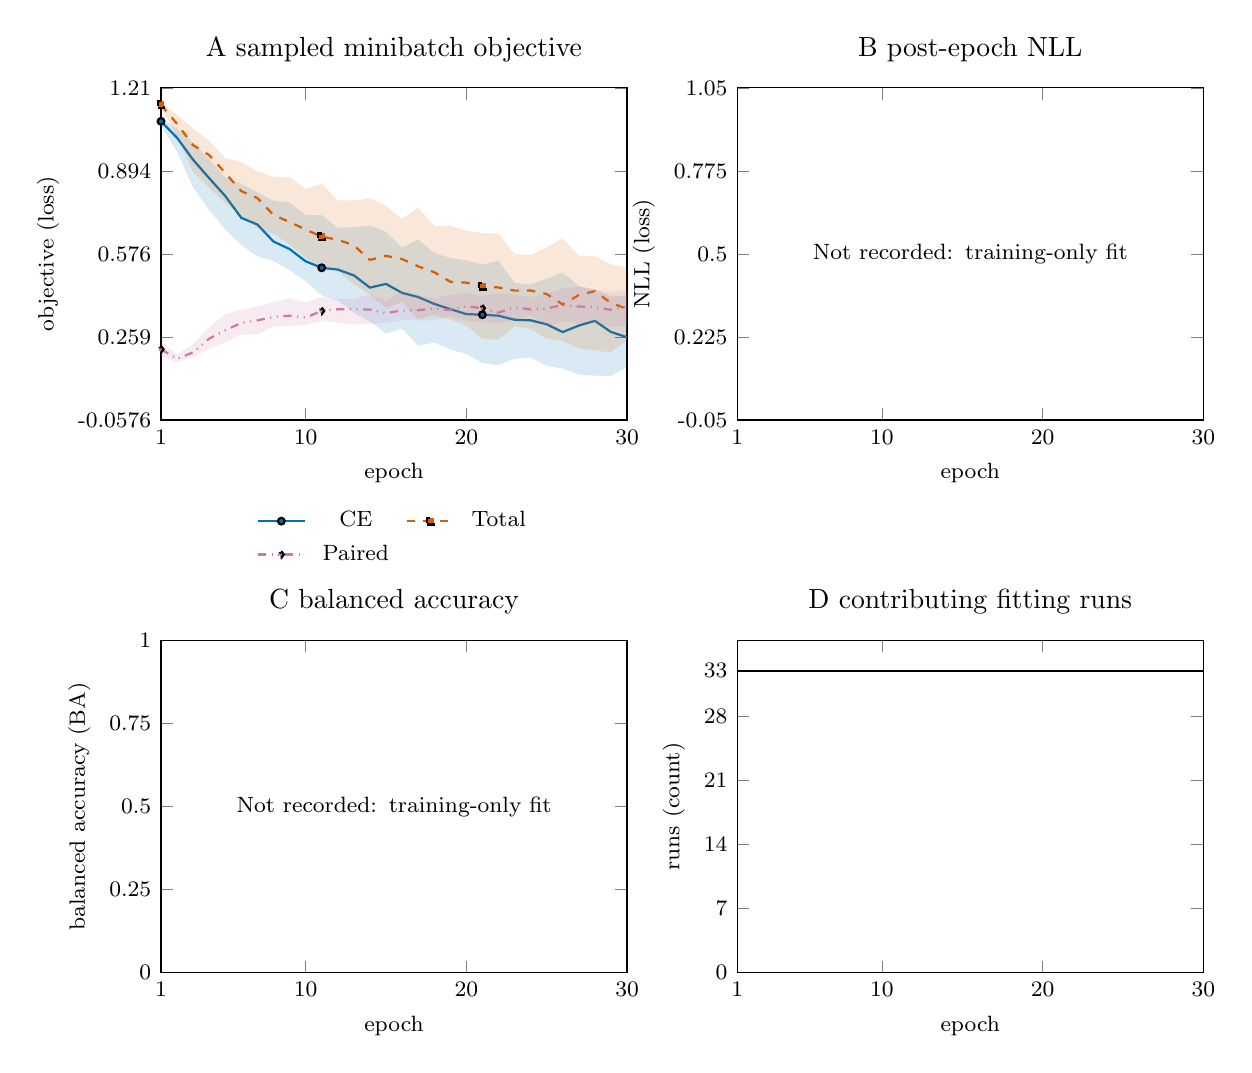
\begin{tikzpicture}
\begin{groupplot}[group style={group size=2 by 2, horizontal sep=14mm, vertical sep=28mm}]
\nextgroupplot[width=75mm, height=58mm, title={A sampled minibatch objective}, xlabel={epoch}, ylabel={objective (loss)}, xmin=1, xmax=30, xtick={1,10,20,30}, ymin=-0.057645774781703955, ymax=1.2105612704157829, ytick={-0.057645774781703955,0.25940598651766772,0.5764577478170394,0.89350950911641103,1.2105612704157829}, yticklabels={-0.0576,0.259,0.576,0.894,1.21}, tick label style={font=\fontsize{8}{9}\selectfont, text=black}, label style={font=\fontsize{8}{9}\selectfont, text=black}, title style={font=\fontsize{10}{11}\selectfont, text=black}, legend style={at={(0.5,-0.24)},anchor=north,draw=none,fill=none,font=\fontsize{8}{9}\selectfont,row sep=1pt,column sep=4pt,legend columns=2}]
\addplot[fill=oi-blue,opacity=0.15,draw=none,forget plot] coordinates {(1,1.0660436570644378) (2,0.96621368825435638) (3,0.83019686639308932) (4,0.7428927600383759) (5,0.66995896995067594) (6,0.61017562150955196) (7,0.56754320561885829) (8,0.54992339611053465) (9,0.51437081098556514) (10,0.47180992513895037) (11,0.41884529888629912) (12,0.39844195991754533) (13,0.35257616937160491) (14,0.31828447282314298) (15,0.27262359559535981) (16,0.29210022985935213) (17,0.22593636065721512) (18,0.2380693256855011) (19,0.2114633485674858) (20,0.19442142844200133) (21,0.15949152670800687) (22,0.15233607739210128) (23,0.17601954266428949) (24,0.18084562048316002) (25,0.14977475777268409) (26,0.13826148994266987) (27,0.1165582574903965) (28,0.11172499209642411) (29,0.11056071780622007) (30,0.14488158449530603) (30,0.41816995888948444) (29,0.41456764489412307) (28,0.43999672979116439) (27,0.4538679361343384) (26,0.50521960556507117) (25,0.48183484822511674) (24,0.46027811169624328) (23,0.46572103649377822) (22,0.55096099078655247) (21,0.53560007214546201) (20,0.55172518789768221) (19,0.56052128970623016) (18,0.58146895915269858) (17,0.63182149529457088) (16,0.60051623880863192) (15,0.65990788042545323) (14,0.68539996147155757) (13,0.67850526869297034) (12,0.6764872252941132) (11,0.72463342249393459) (10,0.72533575594425204) (9,0.77292177081108093) (8,0.77963246405124664) (7,0.81122617125511165) (6,0.84412039816379547) (5,0.86899233460426328) (4,0.9375542551279068) (3,1.0005663633346558) (2,1.0546851098537444) (1,1.094153493642807)};
\addplot[color=oi-blue, mark=*, mark options={draw=black}, mark repeat=10, mark size=1.2pt, solid, line width=0.8pt] coordinates {(1,1.0827530920505524) (2,1.0198495388031006) (3,0.93602095544338226) (4,0.86564426124095917) (5,0.79748150706291199) (6,0.71419374644756317) (7,0.68863548338413239) (8,0.62386983633041382) (9,0.59532558917999268) (10,0.54841019213199615) (11,0.52365311980247498) (12,0.51695329695940018) (13,0.49464657157659531) (14,0.44802242517471313) (15,0.46206522732973099) (16,0.42780536413192749) (17,0.41209403425455093) (18,0.38584176450967789) (19,0.36585555970668793) (20,0.34686172008514404) (21,0.34448840469121933) (22,0.34067895263433456) (23,0.32516536489129066) (24,0.32294759899377823) (25,0.30786028504371643) (26,0.27818703651428223) (27,0.30308228731155396) (28,0.32101073861122131) (29,0.27855511009693146) (30,0.25838994234800339)};
\addlegendentry{CE}
\addplot[fill=oi-vermillion,opacity=0.15,draw=none,forget plot] coordinates {(1,1.1343935370445251) (2,1.024735724925995) (3,0.88936684727668758) (4,0.82931237220764165) (5,0.77099701464176174) (6,0.72055457830429082) (7,0.67623271346092229) (8,0.65313954055309298) (9,0.61283682584762578) (10,0.56168712377548213) (11,0.5262471452355385) (12,0.51269171535968783) (13,0.46002672612667084) (14,0.42228919714689256) (15,0.36962836235761642) (16,0.39310099929571152) (17,0.32779529243707656) (18,0.34340163171291349) (19,0.32578187957406046) (20,0.30322458893060683) (21,0.25316483229398729) (22,0.2484183505177498) (23,0.30019267797470095) (24,0.28906231001019478) (25,0.25379537492990495) (26,0.24445100203156472) (27,0.21524388194084168) (28,0.2083504155278206) (29,0.20069362074136735) (30,0.24744007289409636) (30,0.52439097166061399) (29,0.5367560356855392) (28,0.56833300292491917) (27,0.56901782751083374) (26,0.63526587486267094) (25,0.6018884092569351) (24,0.57143430858850475) (23,0.57689268440008168) (22,0.65449883043766022) (21,0.6563004791736603) (20,0.66537692248821267) (19,0.68367353379726414) (18,0.68375976085662848) (17,0.75355127453804016) (16,0.71074142754077918) (15,0.7589527547359467) (14,0.788853719830513) (13,0.78064835965633395) (12,0.78080316781997683) (11,0.84444981515407569) (10,0.82459036111831663) (9,0.87052046358585355) (8,0.87131414413452146) (7,0.8917373895645142) (6,0.92783735990524296) (5,0.94233430922031403) (4,1.0091832339763642) (3,1.0548101902008056) (2,1.1082484543323516) (1,1.152915495634079)};
\addplot[color=oi-vermillion, mark=square*, mark options={draw=black}, mark repeat=10, mark size=1.2pt, dashed, line width=0.8pt] coordinates {(1,1.1463143229484558) (2,1.0730270147323608) (3,0.99168197810649872) (4,0.9536004364490509) (5,0.88559632003307343) (6,0.81614518165588379) (7,0.78986197710037231) (8,0.72523011267185211) (9,0.69847856462001801) (10,0.66977964341640472) (11,0.64226821064949036) (12,0.63096202909946442) (13,0.60947026312351227) (14,0.55351905524730682) (15,0.5693429708480835) (16,0.55688917636871338) (17,0.52924921363592148) (18,0.50704434514045715) (19,0.47041434794664383) (20,0.4668213278055191) (21,0.45320352911949158) (22,0.44844554364681244) (23,0.4364849328994751) (24,0.43663247674703598) (25,0.42365799844264984) (26,0.38348693400621414) (27,0.41967272758483887) (28,0.43423309177160263) (29,0.38933804631233215) (30,0.36680018156766891)};
\addlegendentry{Total}
\addplot[fill=oi-purple,opacity=0.15,draw=none,forget plot] coordinates {(1,0.18739178478717805) (2,0.16266801208257675) (3,0.1830339938402176) (4,0.21488918364048004) (5,0.23959045484662056) (6,0.26802422404289244) (7,0.26945130228996278) (8,0.29859845191240308) (9,0.30158795416355133) (10,0.30491451174020767) (11,0.31969248354434965) (12,0.31469602435827254) (13,0.30666737556457518) (14,0.310626383125782) (15,0.31394251585006716) (16,0.32340936213731764) (17,0.32223055511713028) (18,0.324050822108984) (19,0.33498099744319915) (20,0.32215604633092881) (21,0.31637548208236693) (22,0.31049040257930755) (23,0.32364941388368607) (24,0.34270648956298827) (25,0.30126229077577593) (26,0.3193412646651268) (27,0.31283456087112427) (28,0.31506001800298689) (29,0.29751961231231688) (30,0.30285920947790146) (30,0.44016404002904891) (29,0.43213472217321397) (28,0.44061953723430636) (27,0.45153738409280775) (26,0.44402953088283537) (25,0.42530817091464995) (24,0.41112700402736663) (23,0.42044927328824999) (22,0.42626771181821826) (21,0.41609603464603423) (20,0.42939653098583219) (19,0.41949592977762223) (18,0.4064843565225601) (17,0.41898690909147263) (16,0.43609453737735748) (15,0.39817360043525696) (14,0.42164832204580305) (13,0.40549754798412324) (12,0.40383650511503222) (11,0.41322728544473647) (10,0.39137974381446838) (9,0.40656796842813492) (8,0.39391459971666337) (7,0.37711973190307618) (6,0.36353993862867356) (5,0.34580442905426023) (4,0.29682117626070975) (3,0.23273631632328035) (2,0.19135598018765448) (1,0.24124991521239281)};
\addplot[color=oi-purple, mark=diamond*, mark options={draw=black}, mark repeat=10, mark size=1.2pt, dash dot dot, line width=0.8pt] coordinates {(1,0.21251796558499336) (2,0.17589326947927475) (3,0.20083127543330193) (4,0.25310757756233215) (5,0.2850169762969017) (6,0.31340189278125763) (7,0.3227618932723999) (8,0.33607897907495499) (9,0.34061382710933685) (10,0.33349885791540146) (11,0.35895727574825287) (12,0.36526117473840714) (13,0.36548182368278503) (14,0.36432706564664841) (15,0.35061795264482498) (16,0.36072275042533875) (17,0.36153707653284073) (18,0.36843397468328476) (19,0.36219838261604309) (20,0.37654043734073639) (21,0.36918044835329056) (22,0.35254845023155212) (23,0.3731653019785881) (24,0.36438262462615967) (25,0.36820539087057114) (26,0.38178758695721626) (27,0.37572713196277618) (28,0.3737114816904068) (29,0.36296684294939041) (30,0.37489651888608932)};
\addlegendentry{Paired}
\nextgroupplot[width=75mm, height=58mm, title={B post-epoch NLL}, xlabel={epoch}, ylabel={NLL (loss)}, xmin=1, xmax=30, xtick={1,10,20,30}, ymin=-0.050000000000000003, ymax=1.05, ytick={-0.050000000000000003,0.22500000000000003,0.5,0.77500000000000002,1.05}, yticklabels={-0.05,0.225,0.5,0.775,1.05}, tick label style={font=\fontsize{8}{9}\selectfont, text=black}, label style={font=\fontsize{8}{9}\selectfont, text=black}, title style={font=\fontsize{10}{11}\selectfont, text=black}]
\node[align=center, text width=55mm, font=\fontsize{8}{9}\selectfont] at (axis cs:15.5,0.5) {Not recorded: training-only fit};
\nextgroupplot[width=75mm, height=58mm, title={C balanced accuracy}, xlabel={epoch}, ylabel={balanced accuracy (BA)}, xmin=1, xmax=30, xtick={1,10,20,30}, ymin=0, ymax=1, ytick={0,0.25,0.5,0.75,1}, yticklabels={0,0.25,0.5,0.75,1}, tick label style={font=\fontsize{8}{9}\selectfont, text=black}, label style={font=\fontsize{8}{9}\selectfont, text=black}, title style={font=\fontsize{10}{11}\selectfont, text=black}]
\node[align=center, text width=55mm, font=\fontsize{8}{9}\selectfont] at (axis cs:15.5,0.5) {Not recorded: training-only fit};
\nextgroupplot[width=75mm, height=58mm, title={D contributing fitting runs}, xlabel={epoch}, ylabel={runs (count)}, xmin=1, xmax=30, xtick={1,10,20,30}, ymin=0, ymax=36.300000000000004, ytick={0,7,14,21,28,33}, yticklabels={0,7,14,21,28,33}, tick label style={font=\fontsize{8}{9}\selectfont, text=black}, label style={font=\fontsize{8}{9}\selectfont, text=black}, title style={font=\fontsize{10}{11}\selectfont, text=black}]
\addplot[color=oi-black, solid, line width=0.8pt] coordinates {(1,33) (2,33) (3,33) (4,33) (5,33) (6,33) (7,33) (8,33) (9,33) (10,33) (11,33) (12,33) (13,33) (14,33) (15,33) (16,33) (17,33) (18,33) (19,33) (20,33) (21,33) (22,33) (23,33) (24,33) (25,33) (26,33) (27,33) (28,33) (29,33) (30,33)};
\end{groupplot}
\end{tikzpicture}
\par\vspace{6mm}
\begin{minipage}{175mm}
{\fontsize{8}{10}\selectfont RQ-S01 / Scope E: descriptive training diagnostics. 400-1800 cm-1 inputs: SG uses impulse replacement and Savitzky-Golay smoothing; arPLS uses impulse replacement and baseline correction; both finish with [0,1] min-max scaling. CE = chemical cross-entropy; SupCon = supervised contrastive; Paired = paired consistency; NLL = negative log-likelihood; BA = balanced accuracy. Authenticated complete monitor histories aggregated across unique fitting jobs into descriptive policy/recipe/stage curves. Curves summarize per-epoch minibatch-weighted training chemical cross-entropy and the composite total optimization objective; these sampled minibatch objectives differ from post-epoch evaluation negative log-likelihood. Auxiliary supcon/paired loss components are recipe-specific and are not directly comparable to the total objective across recipes. Validation metrics are recorded for source\_fit runs only and never substitute for a held-out test set; calibration\_model\_fit and final\_refit rows carry training-only diagnostics. Source\_fit optimization uses a 30-epoch minimum stopping threshold and a 200-epoch maximum; refit stages reuse the caller-selected duration. Curves are fitting-run-weighted descriptive summaries over correlated runs (seeds/splits). Lines show medians; 10th/90th percentiles describe variation among saved fitting runs, not confidence intervals. Only runs that reached each epoch contribute; early stopping changes the composition, and stopped runs are not carried forward. Fitting jobs are not independent chemical samples: the dataset has 598 spectra from 69 physical samples and 10 instruments. Coverage is limited to saved SG/arPLS monitor histories; historical MIN losses are not pooled or invented. A missing history is not a zero loss or proof of a failed model. These curves do not support hypothesis tests, superiority claims, model selection, or new uncertainty inference. P08 learned-method performance is reported elsewhere.}
\end{minipage}
\end{minipage}
\end{document}